\documentclass[11pt,a4paper]{article}

\usepackage{fontspec}
\usepackage[margin=2.2cm]{geometry}
\usepackage{amsmath,amssymb}
\usepackage{booktabs}
\usepackage{float}
\usepackage[font=small,skip=6pt]{caption}
\usepackage{graphicx}
\usepackage{algorithm}
\usepackage[noend]{algpseudocode}
\usepackage{microtype}
\usepackage{enumitem}
\usepackage{xurl}
\usepackage[hidelinks]{hyperref}
\usepackage{tikz}
\usetikzlibrary{positioning}
\setlist[itemize]{itemsep=2pt, topsep=4pt}

\graphicspath{{../plots/}}
\setlength{\intextsep}{8pt plus 2pt minus 2pt}
\newcommand{\repo}{https://github.com/michaelo-ponteski/evolutionary-computation}
\algnewcommand{\LineComment}[1]{\State \(\triangleright\) #1}

\title{Evolutionary Computation\\[0.3em]\large Lab 2: Greedy regret heuristics}
\author{Michał Pokładowski \and Oskar Prusinowski}
\date{October 2026}

\begin{document}
\maketitle

\section{Problem description}

We have a set of $n$ nodes. Each node $j$ has a position on a plane and a cost
$c_j$. We have to choose exactly $k = \lceil n/2 \rceil$ nodes and connect them
into a cycle (a Hamiltonian cycle over the chosen nodes). The goal is to make
the length of the cycle plus the costs of the chosen nodes as small as
possible. If a solution is the list of nodes $\pi = (\pi_1, \dots, \pi_k)$, the
objective is
\[
  f(\pi) \;=\; \sum_{i=1}^{k} d_{\pi_i \pi_{i+1}} \;+\; \sum_{i=1}^{k} c_{\pi_i},
  \qquad \pi_{k+1} \equiv \pi_1 ,
\]
where $d_{ij}$ is the Euclidean distance between nodes $i$ and $j$, rounded to
the nearest integer. So we have to decide two things: \emph{which} nodes to
visit and \emph{in what order}.

Both instances, TSPA and TSPB, have 200 nodes, so every solution has 100 nodes.
We compute the distance matrix once, right after reading an instance. The
algorithms use only this matrix and the node costs, not the coordinates.

\section{Implemented algorithms}

The new methods build a solution in the same way as two methods from Lab~1:
nearest neighbour with insertion at any position of an open path, and greedy
cycle. They differ only in \emph{which node} is inserted in each step. As
before, when node $j$ is inserted between two neighbouring nodes $a$ and $b$,
we add the edges $a \to j$ and $j \to b$ and the cost of $j$, and we
\emph{remove} the edge $a \to b$, so its length is subtracted
(Figure~\ref{fig:insertion}). The objective grows by
\[
  \underbrace{d_{aj} + d_{jb}}_{\text{new edges}}
  \;-\; \underbrace{d_{ab}}_{\text{removed edge}}
  \;+\; \underbrace{c_j}_{\text{node cost}} .
\]

\begin{figure}[H]
\centering
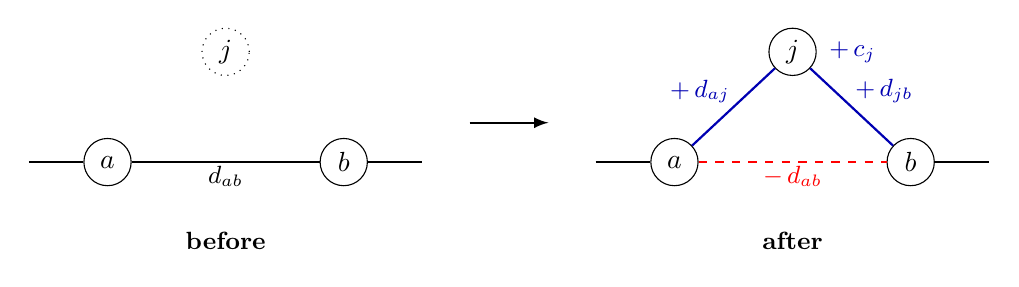
\begin{tikzpicture}[
    node/.style={circle, draw, fill=white, minimum size=6mm, inner sep=0pt},
    edge/.style={thick},
    removed/.style={thick, red, dashed},
    added/.style={thick, blue!70!black},
    lab/.style={font=\small, fill=white, inner sep=1pt}]
  % before
  \node[node] (a1) at (0,0) {$a$};
  \node[node] (b1) at (3,0) {$b$};
  \node[node, dotted] (j1) at (1.5,1.4) {$j$};
  \draw[edge] (-1,0) -- (a1);
  \draw[edge] (b1) -- (4,0);
  \draw[edge] (a1) -- node[lab, below] {$d_{ab}$} (b1);
  \node[font=\small\bfseries] at (1.5,-1) {before};
  % arrow
  \draw[-latex, thick] (4.6,0.5) -- (5.6,0.5);
  % after
  \begin{scope}[xshift=7.2cm]
    \node[node] (a2) at (0,0) {$a$};
    \node[node] (b2) at (3,0) {$b$};
    \node[node] (j2) at (1.5,1.4) {$j$};
    \node[font=\small, text=blue!70!black, right=1pt of j2] {$+\,c_j$};
    \draw[edge] (-1,0) -- (a2);
    \draw[edge] (b2) -- (4,0);
    \draw[removed] (a2) -- node[lab, below, text=red] {$-\,d_{ab}$} (b2);
    \draw[added] (a2) -- node[lab, above left, text=blue!70!black] {$+\,d_{aj}$} (j2);
    \draw[added] (j2) -- node[lab, above right, text=blue!70!black] {$+\,d_{jb}$} (b2);
    \node[font=\small\bfseries] at (1.5,-1) {after};
  \end{scope}
\end{tikzpicture}
\caption{Inserting node $j$ between $a$ and $b$: the edge $a \to b$ (red, dashed) is removed, so its length is subtracted; the edges $a \to j$, $j \to b$ and the cost of $j$ are added (blue).}
\label{fig:insertion}
\end{figure}

For a partial solution $P$ and a node $j \notin P$, let $I(j, P)$ be the list
of the objective changes of all places where $j$ can go:
\begin{itemize}
  \item nearest neighbour (open path $p_1, \dots, p_m$): the beginning
        ($d_{j p_1} + c_j$), the end ($d_{p_m j} + c_j$) and every
        $d_{p_i j} + d_{j p_{i+1}} - d_{p_i p_{i+1}} + c_j$ for every pair of neighbours
        $p_i, p_{i+1}$;
  \item greedy cycle: $d_{aj} + d_{jb} - d_{ab} + c_j$ for every edge $(a, b)$ of the cycle,
        also the one from the last node back to the first.
\end{itemize}
Let $\Delta_1(j)$ and $\Delta_2(j)$ be the smallest and the second smallest
value in $I(j, P)$. The \emph{2-regret} of $j$ is
\[
  r(j) \;=\; \Delta_2(j) - \Delta_1(j) .
\]
It says how much we lose if we do not insert $j$ now and its best place is
taken by another node. The greedy rule from Lab~1 inserts the node with the
smallest $\Delta_1(j)$; the regret heuristics insert the node with the largest
regret, or the largest weighted sum of the regret and the (negative) best
change of the objective. We write both criteria as one score with a weight
$\lambda \in [0, 1]$:
\[
  s_\lambda(j) \;=\; \lambda\, r(j) \;-\; (1 - \lambda)\, \Delta_1(j) .
\]
$\lambda = 1$ is the pure 2-regret, $\lambda = \tfrac12$ gives equal weights,
and $\lambda = 0$ is the greedy rule from Lab~1. The chosen node always goes to
its best place. If two nodes have the same score, we take the one with the
lower index, so each method always gives the same result for the same starting
node.

The greedy cycle versions start from a cycle of two nodes, $s \to j' \to s$.
This cycle uses the edge between $s$ and $j'$ twice, so its objective is
$2 d_{sj'} + c_s + c_{j'}$, and we choose $j'$ with the smallest
$2 d_{sj} + c_j$. In Lab~1 greedy cycle chose it by $d_{sj} + c_j$, which
counts the edge only once; we left the Lab~1 method unchanged, so its results
are the same as in the Lab~1 report. With $\lambda = 0$ the nearest neighbour
version gives exactly the same solutions as Lab~1, and the greedy cycle
version gives the solutions of greedy insertion from this new start (we
checked both in a unit test).

\begin{algorithm}[H]
\caption{Nearest neighbour with greedy 2-regret}
\begin{algorithmic}[1]
\Require starting node $s$
\State $P \gets (s)$ \Comment{an open path $(p_1, \dots, p_m)$}
\While{$|P| < k$}
  \ForAll{$j \notin P$}
    \LineComment{cost of each place where $j$ can go}
    \State $I \gets \bigl(d_{j p_1} + c_j,\; d_{p_m j} + c_j\bigr)$ \Comment{beginning, end}
    \For{$i = 1, \dots, m-1$} \Comment{between neighbours $p_i$ and $p_{i+1}$}
      \State add $d_{p_i j} + d_{j p_{i+1}} - d_{p_i p_{i+1}} + c_j$ to $I$
    \EndFor
    \State $\Delta_1(j), \Delta_2(j) \gets$ the smallest and the second smallest value in $I$
    \State $r(j) \gets \Delta_2(j) - \Delta_1(j)$ \Comment{2-regret}
  \EndFor
  \State $j^\ast \gets \arg\max_{j \notin P} \; r(j)$
  \State insert $j^\ast$ at the place that gives $\Delta_1(j^\ast)$
\EndWhile
\State \Return $P$ \Comment{the last node connects back to the first}
\end{algorithmic}
\end{algorithm}

\begin{algorithm}[H]
\caption{Nearest neighbour with greedy 2-regret + best change of the objective}
\begin{algorithmic}[1]
\Require starting node $s$, weight $\lambda$ (default $\tfrac12$)
\State $P \gets (s)$ \Comment{an open path $(p_1, \dots, p_m)$}
\While{$|P| < k$}
  \ForAll{$j \notin P$}
    \LineComment{cost of each place where $j$ can go}
    \State $I \gets \bigl(d_{j p_1} + c_j,\; d_{p_m j} + c_j\bigr)$ \Comment{beginning, end}
    \For{$i = 1, \dots, m-1$} \Comment{between neighbours $p_i$ and $p_{i+1}$}
      \State add $d_{p_i j} + d_{j p_{i+1}} - d_{p_i p_{i+1}} + c_j$ to $I$
    \EndFor
    \State $\Delta_1(j), \Delta_2(j) \gets$ the smallest and the second smallest value in $I$
    \State $r(j) \gets \Delta_2(j) - \Delta_1(j)$ \Comment{2-regret}
    \State $s(j) \gets \lambda\, r(j) - (1 - \lambda)\, \Delta_1(j)$ \Comment{weighted sum}
  \EndFor
  \State $j^\ast \gets \arg\max_{j \notin P} \; s(j)$
  \State insert $j^\ast$ at the place that gives $\Delta_1(j^\ast)$
\EndWhile
\State \Return $P$ \Comment{the last node connects back to the first}
\end{algorithmic}
\end{algorithm}

\begin{algorithm}[H]
\caption{Greedy cycle with greedy 2-regret}
\begin{algorithmic}[1]
\Require starting node $s$
\State $j' \gets \arg\min_{j \neq s} \; \bigl(2 d_{sj} + c_j\bigr)$ \Comment{objective of $s \to j \to s$}
\State $P \gets (s, j')$ \Comment{an incomplete cycle $s \to j' \to s$}
\While{$|P| < k$}
  \ForAll{$j \notin P$}
    \LineComment{cost of each place where $j$ can go}
    \State $I \gets ()$
    \ForAll{edges $(a, b)$ of $P$} \Comment{also last $\to$ first}
      \State add $d_{aj} + d_{jb} - d_{ab} + c_j$ to $I$
    \EndFor
    \State $\Delta_1(j), \Delta_2(j) \gets$ the smallest and the second smallest value in $I$
    \State $r(j) \gets \Delta_2(j) - \Delta_1(j)$ \Comment{2-regret}
  \EndFor
  \State $j^\ast \gets \arg\max_{j \notin P} \; r(j)$
  \State insert $j^\ast$ at the place that gives $\Delta_1(j^\ast)$
\EndWhile
\State \Return $P$
\end{algorithmic}
\end{algorithm}

\begin{algorithm}[H]
\caption{Greedy cycle with greedy 2-regret + best change of the objective}
\begin{algorithmic}[1]
\Require starting node $s$, weight $\lambda$ (default $\tfrac12$)
\State $j' \gets \arg\min_{j \neq s} \; \bigl(2 d_{sj} + c_j\bigr)$ \Comment{objective of $s \to j \to s$}
\State $P \gets (s, j')$ \Comment{an incomplete cycle $s \to j' \to s$}
\While{$|P| < k$}
  \ForAll{$j \notin P$}
    \LineComment{cost of each place where $j$ can go}
    \State $I \gets ()$
    \ForAll{edges $(a, b)$ of $P$} \Comment{also last $\to$ first}
      \State add $d_{aj} + d_{jb} - d_{ab} + c_j$ to $I$
    \EndFor
    \State $\Delta_1(j), \Delta_2(j) \gets$ the smallest and the second smallest value in $I$
    \State $r(j) \gets \Delta_2(j) - \Delta_1(j)$ \Comment{2-regret}
    \State $s(j) \gets \lambda\, r(j) - (1 - \lambda)\, \Delta_1(j)$ \Comment{weighted sum}
  \EndFor
  \State $j^\ast \gets \arg\max_{j \notin P} \; s(j)$
  \State insert $j^\ast$ at the place that gives $\Delta_1(j^\ast)$
\EndWhile
\State \Return $P$
\end{algorithmic}
\end{algorithm}

The nearest neighbour versions (Algorithms 1 and 2) and the greedy cycle
versions (Algorithms 3 and 4) differ in the start and in the places where a
node can go. In each pair, the weighted version differs from the pure 2-regret
only in the score used to choose the node: $s(j)$ instead of $r(j)$. All four
algorithms look at every place for every node in every step, like the
insertion methods of Lab~1, so they need $O(k^2 n)$ time per solution. We only
have to keep the two best places instead of one.

\section{Computational experiment}

As in Lab~1, we ran each method 200 times, once from every node as the
starting node. 200 solutions take about 1\,s for each regret method, about
twice as long as the greedy insertion methods. To compare the new methods
with the previous ones, we ran all methods from Lab~1 again in the same
experiment (they give the same results as in Lab~1). Table~\ref{tab:results}
shows the objective values of all methods: the methods from Lab~1 (including
200 random solutions) are above the line, the new methods below it. The best
average and the best minimum for each instance are in bold.
Table~\ref{tab:breakdown} shows the median for the new methods and what
their average objective is made of (the same table for the Lab~1 methods is
in the Lab~1 report).

\begin{table}[H]
\centering
\small
\caption{Objective function values over 200 solutions per method. Above the line: methods from Lab~1; below: regret heuristics (this lab).}
\label{tab:results}
\begin{tabular}{lrrrrrr}
\toprule
 & \multicolumn{3}{c}{TSPA} & \multicolumn{3}{c}{TSPB} \\
\cmidrule(lr){2-4}\cmidrule(lr){5-7}
Method & avg & min & max & avg & min & max \\
\midrule
Random & 261\,928 & 236\,759 & 289\,659 & 205\,907 & 174\,617 & 233\,796 \\
NN (end only) & 87\,477 & 84\,362 & 90\,075 & 59\,397 & 56\,007 & 63\,166 \\
NN (any position) & 74\,347 & 72\,328 & 77\,022 & 59\,476 & 52\,915 & 66\,164 \\
Greedy cycle & 73\,797 & 72\,590 & 75\,281 & 59\,709 & 53\,016 & 63\,736 \\
\midrule
NN 2-regret & 122\,861 & 111\,527 & 133\,181 & 74\,763 & 69\,032 & 80\,767 \\
NN 2-regret + change & 75\,554 & 72\,419 & 78\,504 & \textbf{55\,698} & \textbf{50\,485} & 61\,406 \\
Cycle 2-regret & 120\,995 & 112\,654 & 130\,391 & 73\,459 & 69\,609 & 78\,175 \\
Cycle 2-regret + change & \textbf{73\,354} & \textbf{72\,011} & 75\,532 & 57\,866 & 52\,731 & 63\,370 \\
\bottomrule
\end{tabular}

\end{table}

\begin{table}[H]
\centering
\small
\caption{Regret heuristics: median objective, and average cycle length, node costs and closing edge (part of the length).}
\label{tab:breakdown}
\begin{tabular}{lrrrrrrrr}
\toprule
 & \multicolumn{4}{c}{TSPA} & \multicolumn{4}{c}{TSPB} \\
\cmidrule(lr){2-5}\cmidrule(lr){6-9}
Method & median & length & costs & closing & median & length & costs & closing \\
\midrule
NN 2-regret & 123\,254 & 22\,558 & 100\,303 & 1\,490 & 74\,509 & 22\,584 & 52\,179 & 1\,566 \\
NN 2-regret + change & 76\,088 & 23\,344 & 52\,210 & 2\,444 & 55\,949 & 20\,850 & 34\,848 & 3\,083 \\
Cycle 2-regret & 121\,118 & 21\,410 & 99\,585 & 167 & 73\,493 & 21\,416 & 52\,043 & 147 \\
Cycle 2-regret + change & 73\,330 & 21\,175 & 52\,179 & 192 & 57\,042 & 17\,016 & 40\,850 & 156 \\
\bottomrule
\end{tabular}

\end{table}

We also tried other weights in the weighted criterion. Table~\ref{tab:weights}
shows the results for $\lambda$ from 0 (the greedy rule) to 1 (the pure
2-regret); the best average in each column is in bold.

\begin{table}[H]
\centering
\small
\caption{Weighted criterion $s_\lambda(j) = \lambda\, r(j) - (1-\lambda)\,\Delta_1(j)$ for different weights $\lambda$, 200 solutions each.}
\label{tab:weights}
\begin{tabular}{rrrrrrrrr}
\toprule
 & \multicolumn{4}{c}{TSPA} & \multicolumn{4}{c}{TSPB} \\
\cmidrule(lr){2-5}\cmidrule(lr){6-9}
 & \multicolumn{2}{c}{NN} & \multicolumn{2}{c}{cycle} & \multicolumn{2}{c}{NN} & \multicolumn{2}{c}{cycle} \\
\cmidrule(lr){2-3}\cmidrule(lr){4-5}\cmidrule(lr){6-7}\cmidrule(lr){8-9}
$\lambda$ & avg & min & avg & min & avg & min & avg & min \\
\midrule
0.0 & \textbf{74\,347} & 72\,328 & 73\,793 & 72\,590 & 59\,476 & 52\,915 & 59\,650 & 55\,655 \\
0.1 & 74\,495 & 72\,343 & 73\,522 & 72\,430 & 57\,490 & 51\,581 & 59\,040 & 54\,843 \\
0.2 & 74\,994 & 72\,758 & 73\,829 & 72\,430 & 57\,078 & 52\,203 & 56\,385 & 53\,042 \\
0.3 & 75\,303 & 72\,283 & 73\,344 & 72\,347 & 56\,417 & 51\,534 & 55\,982 & 52\,522 \\
0.4 & 74\,879 & 72\,306 & \textbf{73\,277} & 72\,144 & \textbf{53\,740} & 51\,776 & \textbf{55\,548} & 52\,197 \\
0.5 & 75\,554 & 72\,419 & 73\,354 & 72\,011 & 55\,698 & 50\,485 & 57\,866 & 52\,731 \\
0.6 & 76\,187 & 73\,581 & 73\,980 & 72\,217 & 54\,127 & 50\,011 & 57\,797 & 51\,637 \\
0.7 & 76\,454 & 74\,348 & 74\,379 & 72\,682 & 54\,878 & 51\,646 & 58\,975 & 53\,089 \\
0.8 & 79\,795 & 76\,584 & 76\,748 & 73\,880 & 57\,070 & 54\,123 & 57\,160 & 53\,651 \\
0.9 & 90\,959 & 84\,697 & 86\,729 & 80\,972 & 62\,930 & 58\,081 & 61\,804 & 57\,741 \\
1.0 & 122\,861 & 111\,527 & 120\,995 & 112\,654 & 74\,763 & 69\,032 & 73\,459 & 69\,609 \\
\bottomrule
\end{tabular}

\end{table}

\clearpage
\section{Best solutions}

Figures~\ref{fig:tspa} and~\ref{fig:tspb} show the best solution of each new
method. The colour and the size of a node show its cost; nodes that are not in
the solution are faded. The red dashed line is the edge from the last node of
the list back to the first.

\begin{figure}[H]
\centering
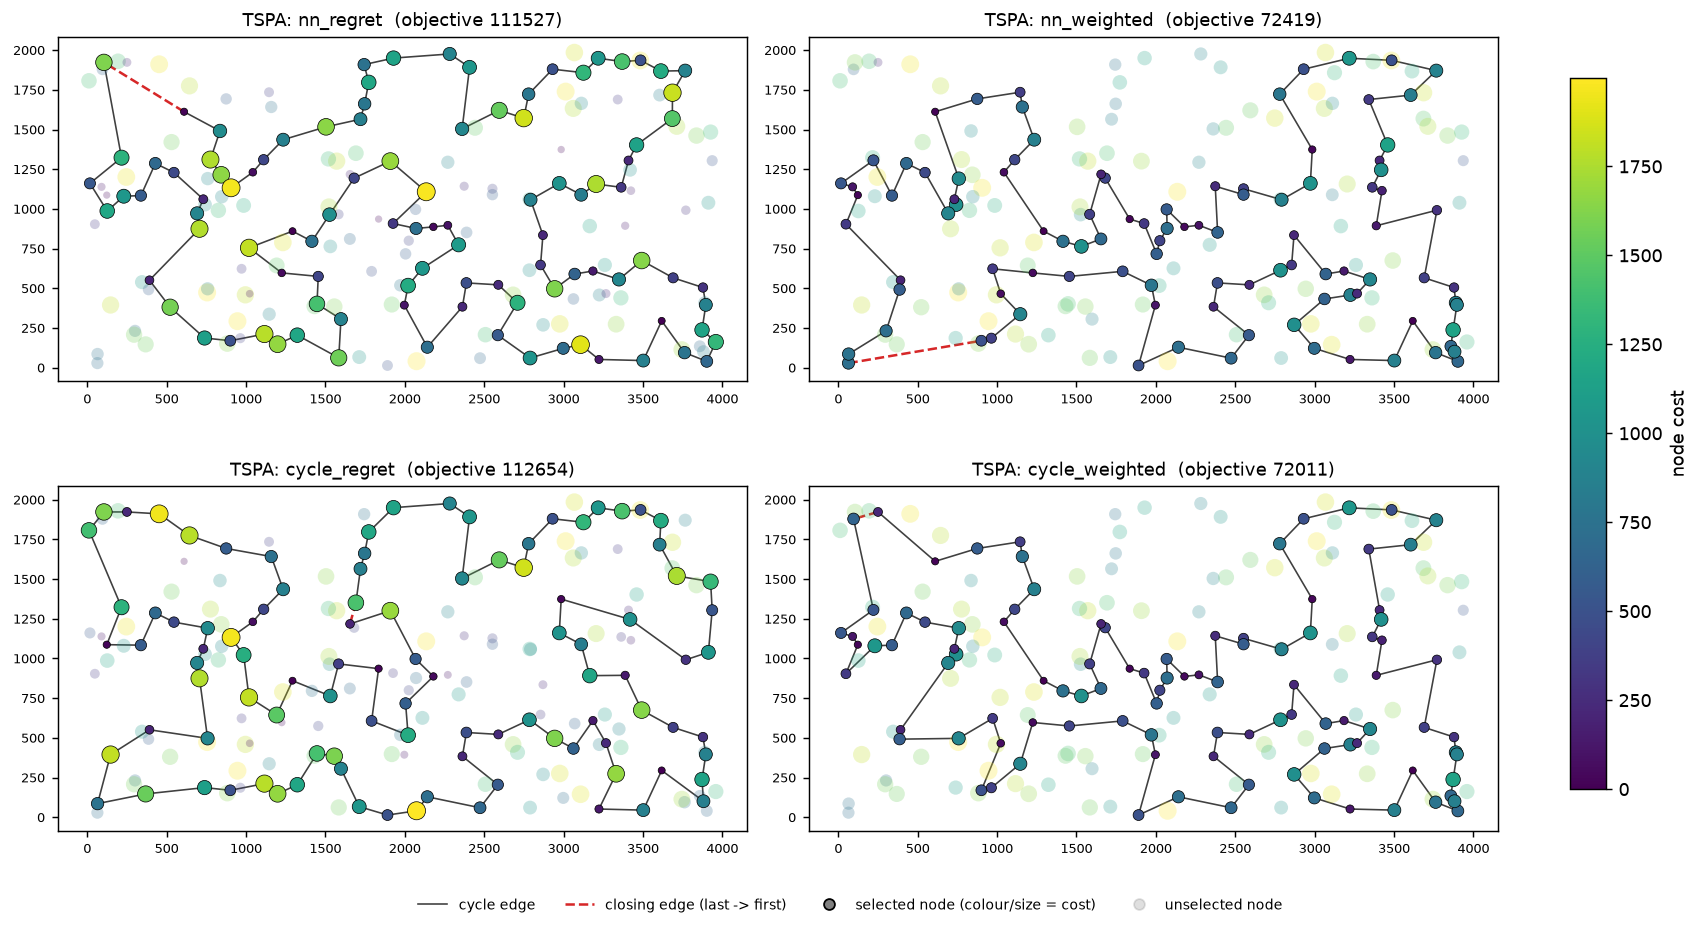
\includegraphics[width=0.93\linewidth]{TSPA.png}
\caption{Best solutions for instance TSPA.}
\label{fig:tspa}
\end{figure}

\begin{figure}[H]
\centering
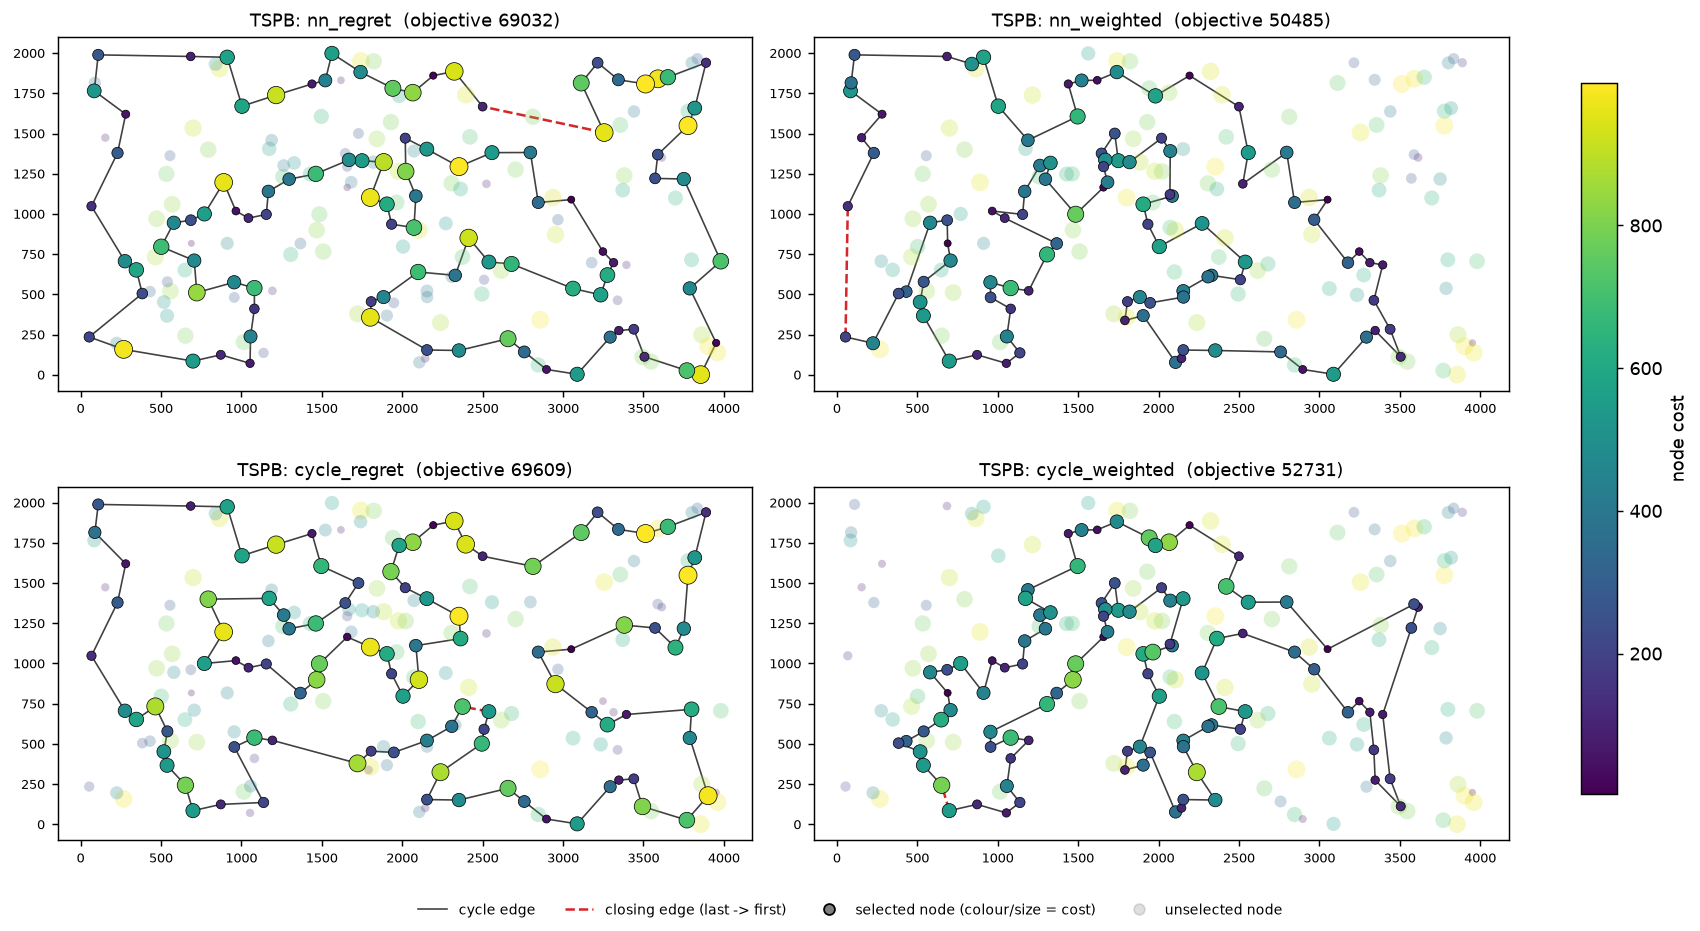
\includegraphics[width=0.93\linewidth]{TSPB.png}
\caption{Best solutions for instance TSPB.}
\label{fig:tspb}
\end{figure}

\subsection*{Best solutions as lists of node indices (starting from 0)}
\paragraph{TSPA, NN 2-regret}
{\footnotesize\ttfamily\raggedright 199, 82, 116, 119, 11, 49, 108, 152, 123, 160, 12, 97, 120, 92, 171, 166, 183, 10, 22, 98, 27, 87, 141, 23, 180, 28, 156, 16, 190, 74, 144, 179, 177, 36, 99, 41, 61, 135, 181, 58, 84, 134, 65, 158, 111, 182, 105, 57, 64, 107, 88, 78, 26, 75, 170, 159, 130, 117, 113, 106, 150, 0, 176, 174, 8, 142, 85, 128, 3, 1, 59, 46, 86, 55, 17, 29, 19, 163, 24, 136, 186, 109, 34, 62, 154, 39, 175, 115, 5, 112, 139, 18, 4, 76, 132, 68, 44, 14, 38, 80\par}

\paragraph{TSPA, NN 2-regret + change}
{\footnotesize\ttfamily\raggedright 171, 2, 189, 187, 30, 141, 87, 45, 73, 135, 114, 181, 192, 158, 58, 84, 134, 72, 176, 174, 150, 106, 113, 89, 42, 151, 138, 182, 57, 64, 107, 88, 78, 193, 153, 75, 170, 146, 159, 130, 47, 93, 50, 3, 169, 1, 59, 178, 101, 55, 29, 163, 136, 186, 164, 142, 8, 9, 54, 33, 131, 36, 177, 52, 179, 53, 140, 144, 67, 16, 51, 35, 185, 102, 28, 180, 132, 76, 4, 71, 157, 91, 80, 100, 123, 83, 160, 152, 108, 49, 60, 116, 149, 63, 168, 97, 127, 69, 129, 104\par}

\paragraph{TSPA, Cycle 2-regret}
{\footnotesize\ttfamily\raggedright 133, 139, 112, 5, 175, 39, 154, 62, 34, 109, 186, 136, 24, 163, 19, 29, 17, 101, 155, 21, 147, 37, 47, 169, 164, 142, 85, 81, 93, 117, 130, 159, 170, 75, 193, 107, 64, 57, 124, 89, 106, 151, 0, 72, 134, 84, 58, 158, 192, 181, 118, 114, 25, 98, 70, 27, 10, 183, 166, 171, 92, 110, 129, 188, 97, 161, 12, 160, 123, 100, 152, 108, 49, 63, 82, 77, 199, 48, 126, 137, 91, 71, 4, 76, 132, 68, 162, 23, 145, 180, 102, 35, 67, 45, 61, 140, 177, 52, 190, 51\par}

\paragraph{TSPA, Cycle 2-regret + change}
{\footnotesize\ttfamily\raggedright 31, 60, 116, 149, 63, 168, 11, 49, 108, 152, 100, 123, 83, 160, 97, 127, 161, 30, 187, 171, 2, 189, 141, 87, 45, 73, 135, 114, 181, 192, 158, 58, 84, 134, 72, 176, 174, 150, 106, 113, 89, 42, 151, 138, 182, 57, 64, 107, 88, 78, 193, 153, 75, 170, 146, 159, 130, 47, 93, 50, 3, 169, 1, 178, 101, 55, 29, 163, 136, 186, 164, 142, 8, 9, 54, 33, 131, 36, 177, 52, 179, 53, 140, 144, 67, 16, 51, 35, 185, 102, 28, 180, 132, 76, 4, 71, 157, 91, 80, 48\par}

\paragraph{TSPB, NN 2-regret}
{\footnotesize\ttfamily\raggedright 57, 44, 89, 32, 43, 48, 58, 198, 121, 195, 50, 42, 116, 37, 13, 149, 145, 65, 178, 103, 132, 1, 108, 62, 175, 134, 157, 60, 141, 155, 113, 115, 19, 177, 125, 26, 161, 154, 140, 47, 38, 21, 168, 136, 8, 95, 128, 122, 151, 111, 3, 137, 72, 86, 0, 185, 104, 162, 54, 127, 129, 52, 182, 150, 84, 66, 35, 24, 25, 73, 59, 101, 179, 88, 163, 99, 171, 17, 74, 20, 14, 2, 93, 23, 110, 118, 131, 148, 10, 196, 193, 61, 105, 169, 165, 199, 70, 190, 194, 12\par}

\paragraph{TSPB, NN 2-regret + change}
{\footnotesize\ttfamily\raggedright 65, 145, 28, 149, 13, 146, 37, 116, 147, 42, 50, 130, 63, 121, 198, 96, 48, 156, 89, 57, 185, 76, 104, 162, 54, 192, 80, 127, 129, 90, 153, 14, 2, 20, 74, 17, 171, 99, 88, 179, 87, 82, 51, 85, 59, 73, 167, 181, 152, 34, 24, 67, 66, 27, 98, 151, 122, 3, 184, 46, 72, 117, 8, 120, 133, 136, 172, 160, 69, 124, 21, 183, 30, 38, 47, 154, 140, 64, 33, 40, 141, 155, 71, 60, 157, 45, 134, 175, 62, 36, 197, 6, 115, 170, 125, 177, 29, 132, 174, 1\par}

\paragraph{TSPB, Cycle 2-regret}
{\footnotesize\ttfamily\raggedright 11, 34, 152, 167, 59, 107, 40, 141, 71, 45, 175, 62, 91, 36, 197, 6, 102, 103, 178, 65, 145, 149, 146, 37, 116, 42, 50, 195, 121, 63, 120, 133, 168, 21, 30, 191, 15, 161, 26, 154, 140, 47, 64, 4, 124, 69, 128, 122, 151, 98, 22, 3, 135, 0, 86, 72, 166, 156, 32, 89, 44, 83, 57, 77, 194, 190, 70, 199, 169, 105, 61, 193, 148, 143, 10, 41, 54, 162, 106, 80, 52, 90, 56, 118, 100, 93, 188, 14, 20, 74, 17, 171, 99, 163, 88, 179, 126, 31, 67, 66\par}

\paragraph{TSPB, Cycle 2-regret + change}
{\footnotesize\ttfamily\raggedright 91, 36, 197, 132, 29, 6, 180, 115, 170, 177, 125, 26, 97, 154, 140, 47, 38, 21, 30, 183, 191, 130, 63, 121, 198, 96, 48, 43, 156, 32, 89, 57, 79, 185, 104, 54, 196, 114, 10, 90, 14, 2, 20, 153, 129, 127, 80, 192, 162, 76, 135, 27, 11, 66, 67, 24, 34, 152, 181, 126, 88, 179, 87, 82, 167, 51, 85, 59, 73, 98, 151, 122, 173, 3, 184, 86, 46, 72, 117, 8, 120, 133, 136, 172, 160, 69, 124, 4, 64, 33, 155, 71, 141, 40, 60, 157, 45, 134, 175, 62\par}


\subsection*{Verification with the solution checker}

We checked all best solutions with the solution checker spreadsheet. We pasted
each list of nodes into the checker, recalculated it and compared its result
with ours (Table~\ref{tab:checker}). All values are the same. We also checked
every solution from the experiment: each one has exactly $k$ different nodes.

\begin{table}[H]
\centering
\small
\caption{Best solutions: our objective value and the value from the checker.}
\label{tab:checker}
\begin{tabular}{lrrrr}
\toprule
 & \multicolumn{2}{c}{TSPA} & \multicolumn{2}{c}{TSPB} \\
\cmidrule(lr){2-3}\cmidrule(lr){4-5}
Method & reported & checker & reported & checker \\
\midrule
NN 2-regret & 111527 & 111527 & 69032 & 69032 \\
NN 2-regret + change & 72419 & 72419 & 50485 & 50485 \\
Cycle 2-regret & 112654 & 112654 & 69609 & 69609 \\
Cycle 2-regret + change & 72011 & 72011 & 52731 & 52731 \\
\bottomrule
\end{tabular}

\end{table}

\section{Source code}

The code is available at \url{\repo/tree/lab2}. It is written in Rust. The
regret heuristics are in \texttt{common/src/heuristics/regret.rs} and use the
same insertion code as the Lab~1 methods (\texttt{insertion.rs}). The
experiment for this lab is in \texttt{lab2/}, and the Python scripts for the
plots and the checker are in \texttt{scripts/}.

\section{Conclusions}

\begin{itemize}
  \item The pure 2-regret is much worse than every greedy method from Lab~1:
        about 121\,000--123\,000 on average on TSPA (vs.\ 73\,800--87\,500) and
        about 73\,500--74\,800 on TSPB (vs.\ about 59\,500). The reason is in
        the definition: the node cost $c_j$ is part of every insertion option
        of $j$, so it cancels out in $r(j) = \Delta_2(j) - \Delta_1(j)$. The
        pure regret does not see the node costs at all. Its cycles are as
        short as the greedy ones (21\,400--22\,600 on TSPA), but the chosen
        nodes cost about 100\,000 on TSPA, slightly more than in random
        solutions (97\,000), while the greedy methods of Lab~1 pay
        51\,000--54\,000 (Table~\ref{tab:breakdown} and the Lab~1 report). In the plots the pure regret solutions
        are full of large, expensive nodes. In our problem, where half of the
        nodes are left out, deciding \emph{which} nodes to take matters as much
        as their order, and the pure regret only looks at the order.
  \item The weighted sum fixes this, because the cost of the node comes back
        through $\Delta_1(j)$. With equal weights, greedy cycle with regret is
        the best method on TSPA (average 73\,354, best 72\,011) and nearest
        neighbour with regret is the best on TSPB (average 55\,698, best
        50\,485). These are the best results of all methods from both labs. On
        TSPB this is a clear gain: 6\,\% better on average than the best Lab~1
        method (nearest neighbour, end only), and the best solution is 4.6\,\% better than the
        best Lab~1 solution. On TSPA the gain is small (0.6\,\% for greedy cycle),
        and nearest neighbour with regret is even 1.6\,\% worse on average than
        without it.
  \item On TSPB the gain of nearest neighbour comes from the node costs. With
        the weighted regret its cycles are longer than without it (20\,850
        vs.\ 18\,678 on average in Lab~1), but its nodes are much cheaper
        (34\,848 vs.\ 40\,798). We think this is the regret at work: a cheap node far
        from the path often has one clearly best place (for example next to
        another cheap node), so its regret is high and it is inserted before
        that place is used. The plain greedy rule postpones such nodes and
        later takes more expensive nodes that are close. Greedy cycle changes
        less on TSPB (node costs 40\,850 vs.\ 41\,774), but its cycles get
        shorter (17\,016 vs.\ 17\,935).
  \item Equal weights are not the best choice (Table~\ref{tab:weights}). The
        results change smoothly with $\lambda$: a small weight of the regret
        ($\lambda = 0.3$--$0.6$) is about as good as or better than
        $\lambda = 0.5$, while from $\lambda = 0.8$ on the results get quickly
        worse, because the node costs count less and less. The best averages
        are at $\lambda = 0.4$ for three of the four combinations (on TSPB:
        53\,740 for nearest neighbour and 55\,548 for greedy cycle). The
        differences between neighbouring weights are not always regular,
        because a small change of the weight changes the order of insertions,
        and the effect of one different decision grows over the next steps.
  \item As in Lab~1, nearest neighbour ignores the edge back to the start, and
        with the weighted regret this edge gets even longer (on average 2\,444
        on TSPA and 3\,083 on TSPB, vs.\ 150--200 in greedy cycle). Even so,
        on TSPB it is the best method; with a better way of closing the cycle,
        or with local search afterwards, it could be better still.
\end{itemize}

\end{document}
